\documentclass[tikz]{standalone}
\usepackage{wasysym}
\usepackage{SIunits}
\usepackage{pgfplots}
\pgfplotsset{compat=1.5}
\usetikzlibrary{plotmarks,arrows}
\tikzset{>=latex}
\definecolor{tissueColour}{RGB}{251,185,130}
\definecolor{lesionColour}{RGB}{175,50,53}
\begin{document}
	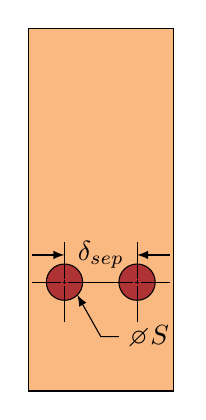
\begin{tikzpicture}[x=0.038\textwidth, y=0.038\textwidth, draw=black, text=black, fill=black]
		% the main domain area
		\draw[fill=tissueColour] (0, 0) rectangle(4, 10);

		% the lesion
		\draw[fill=lesionColour] (1, 3) circle(0.5);
		\draw[fill=lesionColour] (3, 3) circle(0.5);

		% the lesion size
		\draw[<-] (1.354, 2.646) -- (2, 1.5) -- (2.5, 1.5) node[right]{$\diameter S$};
		%\draw (4.1, 4) -- (4.5, 4) node[right]{$\diameter S$};

		% the lesion locators
		\draw (0.1, 3) -- (0.9, 3);
		\draw (1.1, 3) -- (2.9, 3);
		\draw (1, 1.9) -- (1, 2.9);
		\draw (1, 3.1) -- (1, 4.1);
		\draw (1, 2.95) -- (1, 3.05);
		\draw (0.95, 3) -- (1.05, 3);
		\draw (3, 1.9) -- (3, 2.9);
		\draw (3, 3.1) -- (3, 4.1);
		\draw (3.1, 3) -- (3.9, 3);
		\draw (2.95, 3) -- (3.05, 3);
		\draw (3, 2.95) -- (3, 3.05);

		% the lesion separation
		\draw[->] (0.1, 3.75) -- (1, 3.75);
		\draw (2, 3.75) node{$\delta_{sep}$};
		\draw[<-] (3, 3.75) -- (3.9, 3.75);
	\end{tikzpicture}
\end{document}